\section{(2.21)}

We are given the initial wavefunction

\begin{equation}
    \Psi(x,0) = Ae^{-ax^2}.
\end{equation}


\begin{parts}
    

\item Let's find $A$:

\begin{equation*}
    \Braket{\Psi | \Psi} = 2A^2 \int_0^{\infty} e^{-2ax^2}\;\ddx = \frac{2A^2}{\sqrt{2a}} \int_0^{\infty}e^{-u^2}\;\dd u = \frac{2A^2}{\sqrt{2a}} \frac{\sqrt{\pi}}{2} = 1,
\end{equation*}

so

\begin{equation*}
    \boxed{A = \sqrt[4]{\frac{2a}{\pi}}.}
\end{equation*}


\item To find $\Psi(x,t)$, we need to find the coefficient function $\phi(k)$, which can be done using Fourier transforms:

\begin{equation*}
    \phi(k) = \frac{1}{\sqrt{2\pi}} \intinf \Psi(x,0) e^{-ikx} \;\ddx = \sqrt[4]{\frac{2a}{\pi}}\frac{1}{\sqrt{2\pi}} \intinf e^{-(ax^2 + ikx)}\;\ddx.
\end{equation*}

Using the hint from the book, we can ``complete the square'' by making the change of variables:

\begin{equation*}
    u = \sqrt{a} \left( x + \frac{ik}{2a} \right), \quad \mathrm{so} \quad \ddx = \frac{1}{\sqrt{a}}\dd u.
\end{equation*}

Now, to check,

\begin{equation*}
    u^2 + \frac{k^2}{4a} = a\left( x^2 - \frac{k^2}{4a^2} + \frac{ikx}{a} \right) + \frac{k^2}{4a} = ax^2 - \frac{k^2}{4a} + ikx + \frac{k^2}{4a} = ax^2+ikx,
\end{equation*}

which is exactly what we have in our exponential. So,

\begin{align*}
    \phi(k) &= \sqrt[4]{\frac{2a}{\pi}}\frac{1}{\sqrt{2a\pi}} \intinf e^{-(u^2 + k^2/4a)} \;\dd u, \\
    &= \sqrt[4]{\frac{2a}{\pi}}\frac{2}{\sqrt{2a\pi}}e^{-k^2/4a} \int_0^{\infty} e^{-u^2}\;\dd u, \\
    &= \sqrt[4]{\frac{2a}{\pi}}\frac{2}{\sqrt{2a\pi}}e^{-k^2/4a} \frac{\sqrt{\pi}}{2}, \\
    \phi(x) &=  \frac{e^{-k^2/4a}}{(2\pi a)^{1/4}}
\end{align*}

Now,

\begin{align*}
    \Psi(x,t) &= \frac{1}{\sqrt{2\pi}} \intinf \phi(k) e^{i(kx - \frac{\hbar k^2}{2m}t)}\;\dd k, \\
    &= \frac{1}{(2\pi a)^{1/4}\sqrt{2\pi}} \intinf e^{-k^2/4a}e^{i(kx - \frac{\hbar k^2}{2m}t)}\;\dd k, \\
    &= \frac{1}{(2\pi a)^{1/4}\sqrt{2\pi}} \intinf e^{-[(1/4a + i\hbar t/2m)k^2 - ixk]}\;\ddx.
\end{align*}

Doing the same thing as before, we will have

\begin{equation*}
    u = \sqrt{\frac{1}{4a} + \frac{i\hbar t}{2m}}\left[ k - \frac{ix}{(1/2a + i\hbar t/m)} \right], \quad\mathrm{so}\quad \frac{b^2}{4a} = \frac{-x^2}{(1/a + 2i\hbar t/m)},
\end{equation*}

so

\begin{align*}
    \Psi(x,t) &= \frac{1}{(2\pi a)^{1/4}\sqrt{2\pi}} \frac{1}{\sqrt{(1/4a + i\hbar t/2m)}} \intinf e^{-u^2} e^{-x^2/(1/a + 2i\hbar t/m)}\;\ddx, \\
    & \frac{2\sqrt{2} e^{-ax^2/(1 + 2i\hbar at/m)}}{(2\pi a)^{1/4}\sqrt{\pi}}\frac{1}{\sqrt{(1/a + 2i\hbar t/m)}} \int_0^{\infty} e^{-u^2}\;\dd u, \\
    &= \frac{\sqrt{2a} e^{-ax^2/(1 + 2i\hbar at/m)}}{(2\pi a)^{1/4}}\frac{1}{\sqrt{(1 + 2i\hbar at/m)}}, \\
    \Aboxed{ \Psi(x,t) &= \sqrt[4]{\frac{2a}{\pi}}\frac{e^{-ax^2/(1 + 2i\hbar at/m)}}{\sqrt{(1 + 2i\hbar at/m)}}.}
\end{align*}

Using the book's suggestion of $\gamma = \sqrt{1 + 2i\hbar at/m}$:

\begin{equation*}
    \boxed{\Psi(x,t) = \sqrt[4]{\frac{2a}{\pi}} \frac{1}{\gamma} e^{-ax^2/\gamma^2}.}
\end{equation*}


\item Squaring this,

\begin{equation*}
    \abs{\Psi(x,t)}^2 = \sqrt{\frac{2a}{\pi}} \frac{1}{\sqrt{1+(2\hbar at/m)^2}} e^{-ax^2/(1 + 2i\hbar at/m)}e^{-ax^2/(1 - 2i\hbar at/m)}.
\end{equation*}

Looking just at the exponentials real quick:

\begin{equation*}
    -ax^2 \left( \frac{1-2i\hbar at/m + 1+2i\hbar at/m}{1 + (2\hbar at/m)^2} \right) = \frac{-2ax^2}{1 + (2\hbar at/m)^2} - -2\omega^2x^2,
\end{equation*}

with $\omega = \sqrt{a/[(1+(2\hbar at/m)^2)]}$. So,

\begin{equation*}
    \boxed{\abs{\Psi(x,t)}^2 = \sqrt{\frac{2}{\pi}} \omega e^{-2\omega^2x^2}.}
\end{equation*}

\begin{figure}[ht]
    \centering
    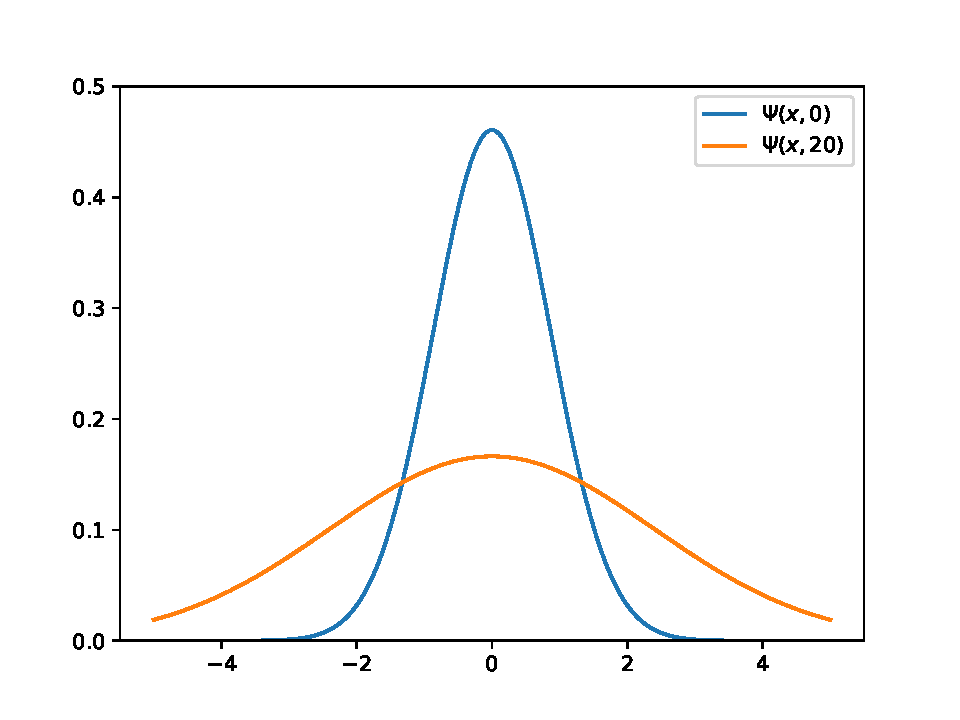
\includegraphics[width=0.4\textwidth]{./res/Prblm4.pdf}
    \caption{Plot of $\abs{\Psi(x,t)}^2$ for time $t=0$ and $t=20$. All constants were taken to be 1 just to get a qualitative picture.}
    \label{fig:Prblm4PsiSquared}
\end{figure}

 



\item Since $\hat{x} = x$ is just a number, we have that:

\begin{equation*}
    \braket{x} = \intinf x \abs{\Psi(x.t)}^2 \;\ddx
\end{equation*}

Since $\Psi \sim e^{-\xi^2}$, we have an odd integrand so $\braket{x}=0$. Similarly, then, $\braket{p} = 0$. Now,

\begin{equation*}
    \Braket{x^2} = \sqrt{\frac{2}{\pi}}w \intinf x^2 e^{-2\omega^2x^2}\;\ddx.
\end{equation*}

With $u = w\sqrt{2} x$, this is

\begin{equation*}
    \Braket{x^2} = \sqrt{\frac{2}{\pi}}\omega \left( \frac{1}{\omega\sqrt{2}} \right)^3 \intinf u^2 e^{u^2}\;\dd u = 2\sqrt{\frac{2}{\pi}}\omega \left( \frac{1}{\omega\sqrt{2}} \right)^3 \frac{\sqrt{\pi}}{4} = \boxed{\frac{1}{4\omega^2}.}
\end{equation*}

Now, $\braket{p^2}$ will be much more challenging:

\begin{equation*}
    \Braket{p^2} = -\hbar^2 \intinf \Psi^* \diff[2]{\Psi}{x} \;\ddx.
\end{equation*}

Doing the derivatives and using the equation for $\Psi$ in terms of $\gamma$:

\begin{equation*}
    \diff[2]{\Psi}{x} = \sqrt[4]{\frac{2a}{\pi}} \frac{1}{\gamma} \diff{}{x} \left[ -\frac{2ax}{\gamma} e^{-ax^2/\gamma^2} \right] = \sqrt[4]{\frac{2a}{\pi}} \frac{1}{\gamma} \left( \frac{4a^2}{\gamma^4}x^2 - \frac{2a}{\gamma^2} \right)e^{-ax^2/\gamma^2}.
\end{equation*}

So,

\begin{align*}
    \Braket{p^2} = -\hbar^2 \sqrt{\frac{2}{\pi}} \frac{\sqrt{a}}{\gamma^*\gamma}  \intinf \left( \frac{4a^2}{\gamma^4}x^2 - \frac{2a}{\gamma^2} \right)e^{-ax^2/(\gamma^2)^*}e^{-ax^2/\gamma^2} \;\ddx.
\end{align*}

Now, let's look at this term:

\begin{equation*}
    \frac{\sqrt{a}}{\gamma^*\gamma} = \frac{\sqrt{a}}{\sqrt{(1-2i\hbar at/m)(1+2i\hbar at/m)}} = \frac{\sqrt{a}}{\sqrt{1+(2\hbar at/m)^2}} = \omega,
\end{equation*}

and the exponentials will look similar as well; they become what we got for $\Psi$ in terms of $\omega$. Thus,

\begin{align*}
    \Braket{p^2} &= \frac{2a\hbar^2}{\gamma^2} \sqrt{\frac{2}{\pi}} \omega \intinf \left( 1 - \frac{2a}{\gamma^2}x^2 \right)e^{-2\omega^2x^2}\;\ddx, \\
    &= \frac{4a\hbar^2}{\gamma^2} \sqrt{\frac{2}{\pi}} \omega \left[ \int_0^{\infty} e^{-2\omega^2x^2}\;\ddx -\frac{2a}{\gamma^2}\int_0^{\infty}x^2e^{-2\omega^2x^2}\;\ddx \right], \\
    &= \frac{4a\hbar^2}{\gamma^2} \sqrt{\frac{2}{\pi}} \omega \left[ \left( \frac{1}{\omega\sqrt{2}} \right) \int_0^{\infty} e^{-u^2}\;\dd u - \frac{2a}{\gamma^2}\left( \frac{1}{\omega\sqrt{2}} \right)^3 \int_0^{\infty} u^2e^{-u^2}\;\dd u \right], \\
    &= \frac{4a\hbar^2}{\gamma^2} \sqrt{\frac{2}{\pi}} \left[ \frac{1}{\sqrt{2}}\left( \frac{\sqrt{\pi}}{2} \right) -  \frac{2a}{\gamma^2} \frac{1}{2\omega^2\sqrt{2}}\left( \frac{\sqrt{\pi}}{4} \right) \right], \\
    &= \frac{2a\hbar^2}{\gamma^2} \left( 1 - \frac{a}{2\gamma^2\omega^2} \right).
\end{align*}

Looking at the term in parentheses:

\begin{align*}
    1 - \frac{a\left[ 1+(a\hbar at/m)^2 \right]}{2a(1+2i\hbar at/m)} = 1- \frac{(1+2i\hbar at/m)(1i2i\hbar at/m)}{2(1+2i\hbar at/m)} = 1- \frac{1-2i\hbar at/m}{2} = \frac{1+2i\hbar at/m}{2} = \frac{\gamma^2}{2},
\end{align*}

So,

\begin{equation*}
    \boxed{\Braket{p^2} = a\hbar^2.}
\end{equation*}

Therefore, we have that

\begin{equation*}
    \sigma_x = \sqrt{\frac{1}{4\omega^2}} = \frac{1}{2\omega}, \ \mathrm{and} \ \sigma_p = \sqrt{a\hbar^2} = \hbar \sqrt{a}.
\end{equation*}


\item From this, we can say

\begin{equation*}
    \sigma_x\sigma_p = \frac{\hbar}{2}\frac{\sqrt{a}}{\omega} = \frac{\hbar}{2} \sqrt{[1+(2\hbar at/m)^2]}.
\end{equation*}

The square root will allways be greater than one since the quantity in parentheses will always be positive. We can see that for $t=0$, this comes exactly to the uncertainty limit.


\end{parts}